\documentclass{article}

\usepackage{fancyhdr}
\usepackage{extramarks}
\usepackage{amsmath}
\usepackage{amsthm}
\usepackage{amsfonts}
\usepackage{tikz}
\usepackage[plain]{algorithm}
\usepackage{algpseudocode}
\usepackage{enumerate}
\usepackage{tikz}
\usepackage{pythonhighlight}
\usetikzlibrary{automata,positioning}

%
% Basic Document Settings
%  

\topmargin=-0.45in
\evensidemargin=0in
\oddsidemargin=0in
\textwidth=6.5in
\textheight=9.0in
\headsep=0.25in

\linespread{1.1}

\pagestyle{fancy}
\lhead{\hmwkAuthorName}
\chead{\hmwkClass : \hmwkTitle}
\rhead{\firstxmark}
\lfoot{\lastxmark}
\cfoot{\thepage}

\renewcommand\headrulewidth{0.4pt}
\renewcommand\footrulewidth{0.4pt}

\setlength\parindent{0pt}

%
% Create Problem Sections
%

\newcommand{\enterProblemHeader}[1]{
    \nobreak\extramarks{}{Problem \arabic{#1} continued on next page\ldots}\nobreak{}
    \nobreak\extramarks{Problem \arabic{#1} (continued)}{Problem \arabic{#1} continued on next page\ldots}\nobreak{}
}

\newcommand{\exitProblemHeader}[1]{
    \nobreak\extramarks{Problem \arabic{#1} (continued)}{Problem \arabic{#1} continued on next page\ldots}\nobreak{}
    \stepcounter{#1}
    \nobreak\extramarks{Problem \arabic{#1}}{}\nobreak{}
}

\newcommand*\circled[1]{\tikz[baseline=(char.base)]{
		\node[shape=circle,draw,inner sep=2pt] (char) {#1};}}


\setcounter{secnumdepth}{0}
\newcounter{partCounter}
\newcounter{homeworkProblemCounter}
\setcounter{homeworkProblemCounter}{1}
\nobreak\extramarks{Problem \arabic{homeworkProblemCounter}}{}\nobreak{}

%
% Homework Problem Environment
%
% This environment takes an optional argument. When given, it will adjust the
% problem counter. This is useful for when the problems given for your
% assignment aren't sequential. See the last 3 problems of this template for an
% example.
%

\newenvironment{homeworkProblem}[1][-1]{
    \ifnum#1>0
        \setcounter{homeworkProblemCounter}{#1}
    \fi
    \section{Problem \arabic{homeworkProblemCounter}}
    \setcounter{partCounter}{1}
    \enterProblemHeader{homeworkProblemCounter}
}{
    \exitProblemHeader{homeworkProblemCounter}
}

%
% Homework Details
%   - Title
%   - Class
%   - Due date
%   - Name
%   - Student ID

\newcommand{\hmwkTitle}{Homework\ \#01}
\newcommand{\hmwkClass}{Probability \& Statistics for EECS}
\newcommand{\hmwkDueDate}{Feb 29, 2024}
\newcommand{\hmwkAuthorName}{Fei Pang}
\newcommand{\hmwkAuthorID}{2022533153}


%
% Title Page
%

\title{
    \vspace{2in}
    \textmd{\textbf{\hmwkClass:\\  \hmwkTitle}}\\
    \normalsize\vspace{0.1in}\small{Due\ on\ \hmwkDueDate\ at 23:59}\\
	\vspace{4in}
}

\author{
	Name: \textbf{\hmwkAuthorName} \\
	Student ID: \hmwkAuthorID}
\date{}

\renewcommand{\part}[1]{\textbf{\large Part \Alph{partCounter}}\stepcounter{partCounter}\\}

%
% Various Helper Commands
%

% Useful for algorithms
\newcommand{\alg}[1]{\textsc{\bfseries \footnotesize #1}}
% For derivatives
\newcommand{\deriv}[1]{\frac{\mathrm{d}}{\mathrm{d}x} (#1)}
% For partial derivatives
\newcommand{\pderiv}[2]{\frac{\partial}{\partial #1} (#2)}
% Integral dx
\newcommand{\dx}{\mathrm{d}x}
% Alias for the Solution section header
\newcommand{\solution}{\textbf{\large Solution}}
% Probability commands: Expectation, Variance, Covariance, Bias
\newcommand{\E}{\mathrm{E}}
\newcommand{\Var}{\mathrm{Var}}
\newcommand{\Cov}{\mathrm{Cov}}
\newcommand{\Bias}{\mathrm{Bias}}

\begin{document}

\maketitle

\pagebreak

\begin{homeworkProblem}[1]

\begin{enumerate}[(1)]
    % inline
    \item 
    Consider we are forming $k$ groups of $n+1$ people and I am among the $n+1$ people. 
    There are two possibilites: the other $n$ people form $k-1$ groups and I am in a group by myself,
    \ or the other $n$ people form $k$ groups already, so I only have to join one of the k groups. 
    
    
    \item
    Consider we are forming $k+1$ groups of $n+1$ people and I am among the $n+1$ people.
    There possibilities that $1$, $2$,\(\cdots\), k people are not in my group. So we can divide it into k circumstances
    and the j people(not in my group) form $k$ groups and I lead a group myself.
    
    % \item
   	% \begin{math}
   	% 	f(n)
    % \end{math}
    
    % % Display mode
    % \item
    % \[
    % 	f(n)
    % \]
    
    % \item 
    % $$ 
    % 	f(n)
    % $$
    
    % \item
    % \begin{equation}
    %     	f(n)
    % \end{equation}
\end{enumerate}

\end{homeworkProblem}

\begin{homeworkProblem}[2]

    There are \(P_{26}^{26}\) \emph{norepeatword}s with 26 alphabets,\ and \(P_{26}^{1} + P_{26}^{2} + \cdots \) \emph{norepeatword}s.
    \[P = \frac{P_{26}^{26}}{P_{26}^{1} + P_{26}^{2} + \cdots + P_{26}^{26}}\]
    \[\frac{1}{P}=1+\frac{1}{2!}+\frac{1}{3!}+\frac{1}{4!}+\cdots+\frac{1}{25!}=\sum_{n=1}^{25}\frac{1}{n!} \approx \sum_{i=1}^{\infty} \frac{1}{n!} = e\]
    \[So\ P \approx \frac{1}{e}.\]
% \begin{enumerate}
% 	% alignment
% 	\item
%     \[
%     	\begin{split}
% 	    		n^{2} + n + 1 
% 	    		\le ~& n^{2} + n^{2} + n^{2} \\
% 	    		= ~& 3 n^{2} \\
% 	    		\le ~& c \cdot 2 n^{3}
% 	    	\end{split}
%     \]
    
%     \item
%     \begin{equation}
%     	\begin{aligned}
% 	    		n^{2} + n + 1 
% 	    		\le ~& n^{2} + n^{2} + n^{2} \\
% 	    		= ~& 3 n^{2} \\
% 	    		\le ~& c \cdot 2 n^{3}
% 		\end{aligned}
% 	\end{equation}
	
% 	\item
% 	\begin{align}
% 	    	n^{2} + n + 1 
% 	    	\le ~& n^{2} + n^{2} + n^{2} \\
% 	    	= ~& 3 n^{2} \\
% 	    	\le ~& c \cdot 2 n^{3}
% 	\end{align}
% \end{enumerate}

\end{homeworkProblem}

\begin{homeworkProblem}[3]
    \begin{enumerate}[(a)]
        \item Apparently,\ we have \(n^n\) possible bootstrap samples.
        \item Assume \((a_1, a_2, \cdots a_n)\)\ and\ \((b_1, b_2, b_3, \cdots b_n)\).\\
        Each \(b_n\) presents the number of times that each \(a_n\) is chosen.\ So\ \(\sum_{i=1}^{n} b_i = n\).
        
        Then it turns out to be a partition problem:\ We should put \(n-1\) partitions to seperate the numbers into k different boxes.
        So,\ there are \(2n - 1\) places to be inserted,\ which is a \(\binom{2n - 1}{n - 1}\).
        So there are \(\frac{(2n-1)!}{n!(n-1)!}\)kinds.
        
        \item Assume the bootstrap samples have orders so there are \(n^n\) kinds.

        
        \(b1\): only one kind:\({a_1,a_1,a_1\cdots,a_1}\).\\
        \(b2\): each number appears once: \(a_1,a_2,a_3\cdots a_n\) is \(n!\).
        
        So \(p_1=\frac{n!}{n^n},\ p_2=\frac{1}{n^n}\). \(\frac{p_1}{p_2} = n!\)
        
        Probability of getting \(p_1\): \(\frac{n!}{n^n}\).

        probability of getting \(p_2\): \( n\times\frac{1}{n^n}\).

        The ratio is \((n-1)!\)
    \end{enumerate}

\end{homeworkProblem}

\begin{homeworkProblem}[4]
    
    
    Assume the length of the stick is \(k\) and the three pieces are \(a\),\ \(b\),\ and \(k - a - b\). To form a triangle, we have to satisfy:
    \begin{equation}
    \begin{split}
    a + b &> k - a - b\\
    a + k - a - b &> b \notag\\
    b + k - a - b &> a 
    \end{split}
    \end{equation}
    The fig below gives a way to calculate the possibility, which is the proportion of the area of the shadow.
    \[So\  P = \frac{1}{4}.\] 
    \begin{figure}[htbp]
        \centering
        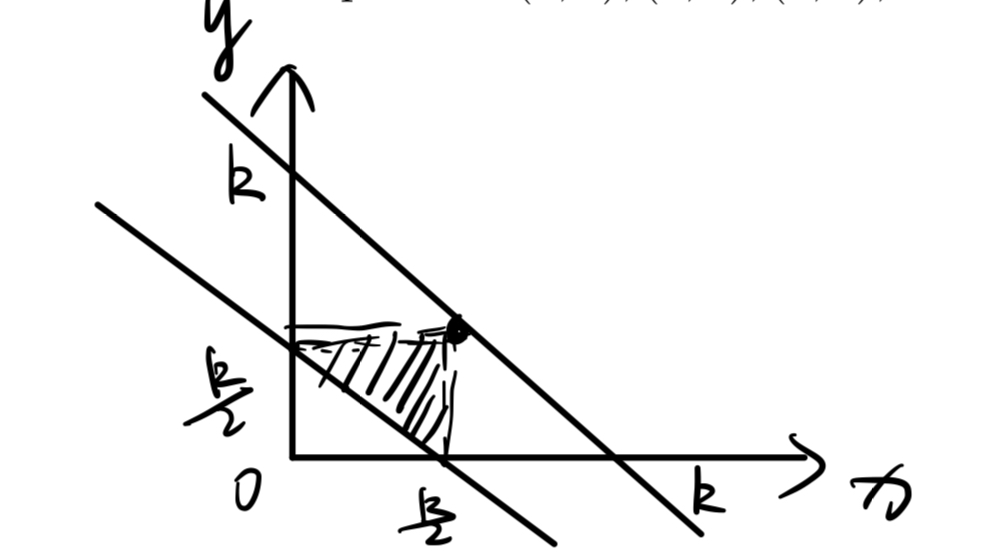
\includegraphics[width=0.4\columnwidth,height=0.2\linewidth]{P4_fig.jpg}
        \caption{LP}
    \end{figure} 
  
\end{homeworkProblem}

\begin{homeworkProblem}[5]
    \begin{enumerate}[(a)]
        \item There are \(k\) people,then the probability of at least one holiday
        match is
        \[1-k!e_k(p_1,p_2,p_3,\cdots,p_{365})=1-k!e_k(\vec{p}).\]
        
        \item Consider \(k=2,P=1-2e_2(\vec{p})=\sum^{365}_{j=1}p_j^2\geq\frac{(p_1+p_2+\cdots+p_{365})^2}{365}\)\\
        We know that it is only equal when \(p_1=p_2=\cdots=p_{365}=\frac{1}{365}\).

        \item 

        1: A's birthday is on 1 day,B's birthday is on another day, others' don't match
        and are not on day1 or day2 \(\Rightarrow x_1x_2e_{k-2}(x_3\cdots,x_n)\)
        
        2:A's birthday and B's birthday are on one day, others' on another day \(\Rightarrow (x_1+x_2)e_{k-1}(x_3,\cdots,x_n)\)
        
        3:All people's birthday don't match.
        
        So we have
        \(e_k(x_1\cdots,x_n)=x_1x_2e_{k-2}(x_3\cdots,x_n)+(x_1+x_2)e_{k-1}(x_3,\cdots,x_n)+e_k(x_3\cdots,x_n)\).
     
        
        \(e_k(\vec p)=p_1p_2e_{k-2}(p_3\cdots,p_n)+(p_1+p_2)e_{k-1}(p_3,\cdots,p_n)+e_k(p_3\cdots,p_n)\\
        e_k(\vec r)= \frac{(p_1+p_2)^2}{4}e_{k-2}(p_3\cdots,p_n) 
        +(p_1+p_2)e_{k-1}(p_3,\cdots,p_n)+e_k(p_3\cdots,p_n)\\\)
        
        refer to\(\displaystyle\frac{x+y}{2}\geq\sqrt{xy}\) (only equal when
        x=y)
        \[so\ e_k(\vec{p})\leq e_k(\vec{r}),only\ equal\ when\ p_1=p_2\]
        
        So \(P(at\ least\ one\ birthday\ match | p) \geq P(at\ least\ one\ birthday\ match\ |\ r)\).
        
        then we define a vector \(\vec{r}=(r_1,r_2,p_3,p_4,p_5,\cdots)\),
        \(\vec{m}=(r_1,m_2,m_3,p_4,p_5,\cdots),m_2=m_3=\frac{r_2+p_3}{2}\)
        
        \[so\ e_k(\vec{r})\leq e_k(\vec{m}),only\ equal\ when\ m_2=m_3=\frac{p_3+r_2}{2}=\frac{p_3+\frac{p_1+p_2}{2}}{2}\]
        
        then
        \(e_k(\vec{p})\leq e_k(\vec{r})\leq e_k(\vec{m})\leq\cdots e_k(\vec{P})\).
        
        So only equal when \(P_{n+1}=\frac{P_n+P_{n-1}}{2}\),and
        \(P_{1}=\frac{P_{365}+P_{364}}{2}\)
        
        \(\displaystyle\sum^{365}_{k=1}P_j=1\Rightarrow P_j=\frac{1}{365}\)
        
        So \(e_k(\vec{P})\)is max value and the value of p that minimizes the probability of at least one
        birthday match is given by \(p_j = 365\) for all \(j\).
        
    \end{enumerate}
\end{homeworkProblem}

\begin{homeworkProblem}[6]
    
\[P=\frac{108!\begin{Bmatrix}
    n\\108
\end{Bmatrix}}{108^n}
=\frac{\displaystyle\sum^{108}_{k=0}(-1)^kC_{108}^k(108-k)^n}{108^n}
=\displaystyle\sum^{108}_{k=0}(-1)^kC_{108}^k(\frac{108-k}{108})^n\]

Then we use python to plot an image:
\begin{python}

    import numpy as np
    import matplotlib.pyplot as plt
    from scipy.special import comb
    
    def P_function(n):
        result = 0
        for k in range(109):
            result += (-1)**k * comb(108, k) * ((108 - k) / 108)**n
        return result
    
    n_values = np.arange(200, 1001)
    P_values = [P_function(n) for n in n_values]
    
    first_index_above_095 = next((i for i, p in enumerate(P_values) if p > 0.95), None)
    n_value_above_095 = n_values[first_index_above_095]
    
    plt.figure(figsize=(10, 6))
    plt.plot(n_values, P_values, color='blue', linestyle='-')
    plt.scatter(n_value_above_095, P_values[first_index_above_095], color='red', label=f'n={n_value_above_095}')
    plt.xlabel('n', fontsize=14)
    plt.ylabel('P', fontsize=14)
    plt.title('Graph of P for n in the range [200, 1000]', fontsize=16)
    plt.grid(True)
    plt.legend()
    plt.show()
    
\end{python}

\begin{figure}[htbp]
    \centering
    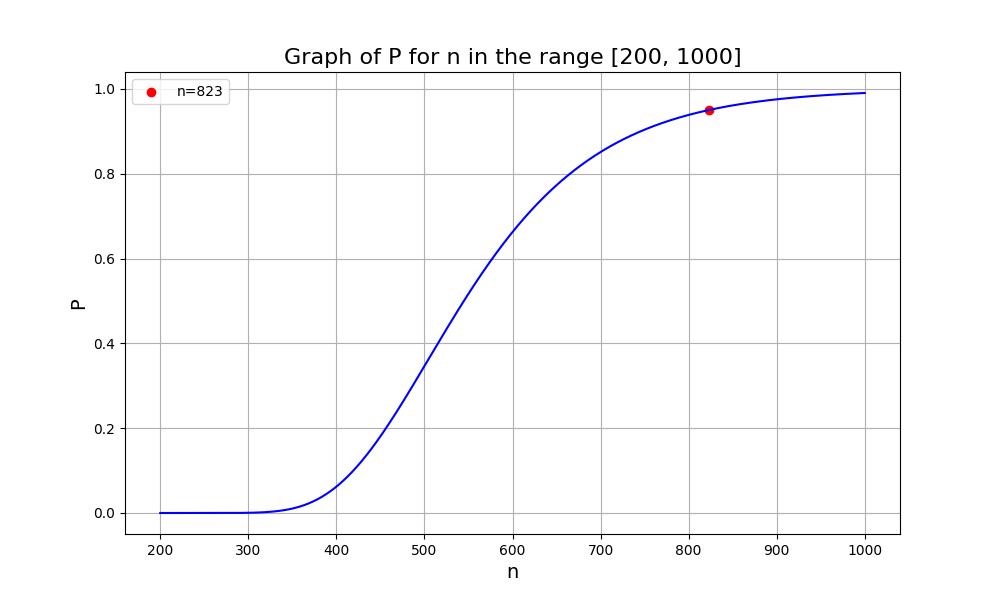
\includegraphics[width=0.5\columnwidth,height=0.3\linewidth]{P6_fig.png}

\end{figure} 
We can tell from the fig that the minimum number of n is 823 when such probability is no less than 95\%.
\end{homeworkProblem}
\end{document}
